\documentclass[10pt,conference]{IEEEtran}


\usepackage[utf8x]{inputenc}
 %\usepackage{fontspec}
\usepackage{ucs}
\usepackage{amsmath}
\usepackage{amssymb}
\usepackage{graphicx}
\usepackage{amsfonts}
\usepackage{textcomp}

\usepackage{multirow}

 \usepackage{psfrag}

\usepackage[T1]{fontenc}

\begin{document}

	\title{Elektrosztatikus mérés szimulációja multiprocesszoros környezetben}
	
	\author{
		\IEEEauthorblockN{Bakró-Nagy~István} \IEEEauthorblockA{ Szélessávú
		Hírközlés és Villamosságtan Tanszék\\ Budapesti Műszaki és Gazdaságtudományi
		Egyetem \\ Budapest \\ \texttt{bakro.istvan@gmail.com}} 
		\and
		\IEEEauthorblockN{Reichardt András} \IEEEauthorblockA{Szélessávú Hírközlés és
		Villamosságtan Tanszék\\ Budapesti Műszaki és Gazdaságtudományi Egyetem \\
		Budapest \\ \texttt{reich@evt.bme.hu}}
	}
	
	\maketitle

	\begin{abstract}
	 Fémezett, töltött felület felett lévő fémtűre ható erő számítását végeztük el.
	 A szimulációk során a lehetséges párhuzamosításokat felhasználva a számítási időt csökkentettük.
	 Kidolgoztunk egy egyszerű szimulációs keretrendszert a felületmérés pontatlanságainak kiegyensúlyozására, az elérhető felbontás javítására.
	\end{abstract}

	\begin{IEEEkeywords}
	 numerikus szimuláció, parallel computing, OpenCL, AFM 
	\end{IEEEkeywords}

	
	\section{Bevezetés}
	1986-ban Binning demonstrálta az atomerő mikroszkóp (AFM) ötletét \cite{Binnig1986}, ami mára 
	a nanotechnológia egyik legfontosabb eszköze lett. Felhasználható képalkotásra, nanolitográfiára és 
	adott anyag alakítására \cite{Vasic2013}.
	Az AFM apparátusa az adott minta felülete és a felette pásztázó kantilever végére erősített tű 
	kölcsönhatásának vizsgálatát végzi. (lásd \ref{fig:tip-sample}. ábra)
	A felület és a tű közötti domináns kölcsönhatás határozza meg, hogy az anyag melyik fizikai
	mennyiségét kaphatjuk meg.
	\begin{figure}[H]
		\centering
		\subfloat[Az AFM apparátusa]{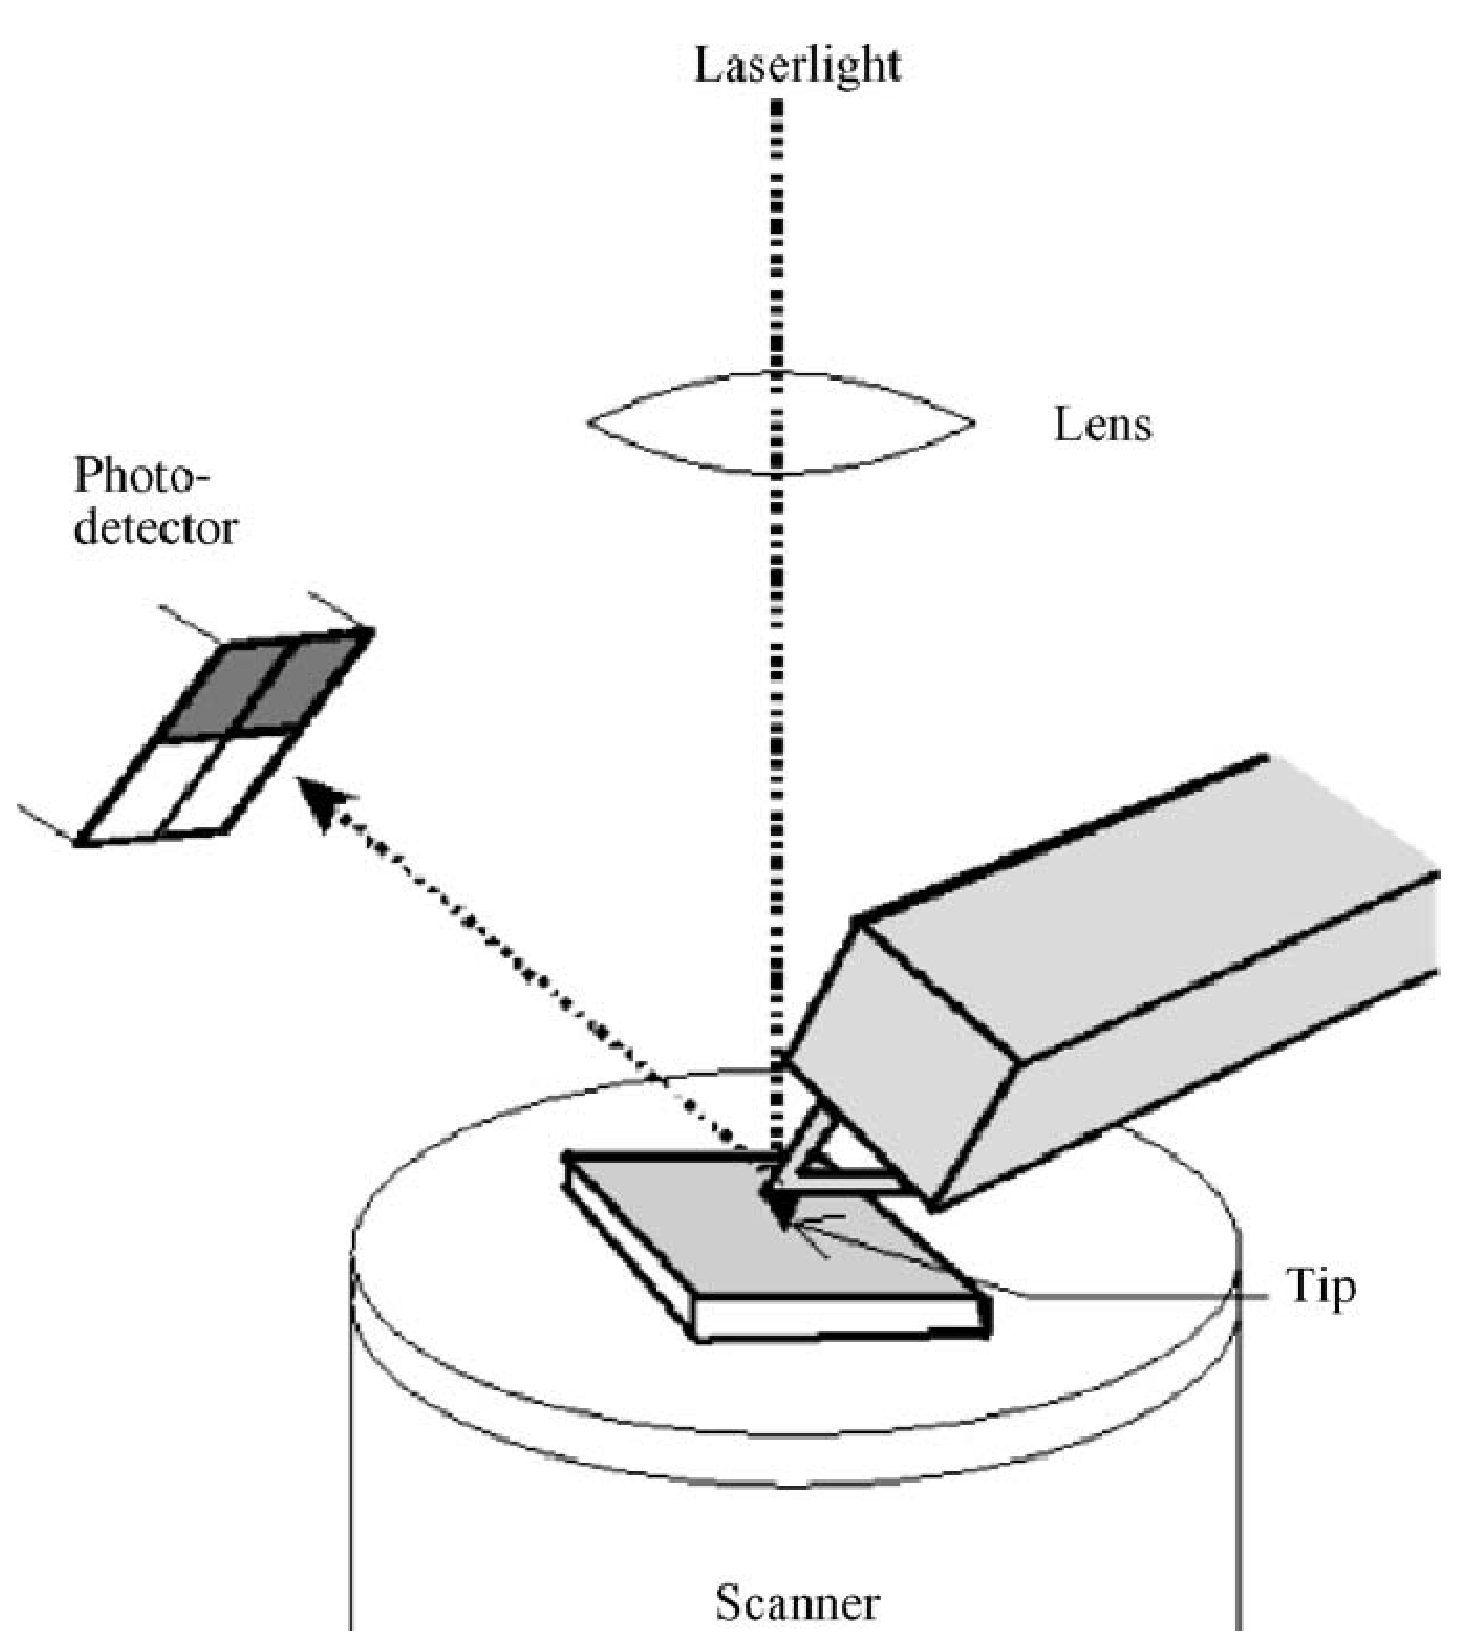
\includegraphics[width=0.45\columnwidth]{kepek/eps/AFM.eps}%
		\label{fig:afm}}
		\hfil
		\subfloat[A tű és minta modellje]{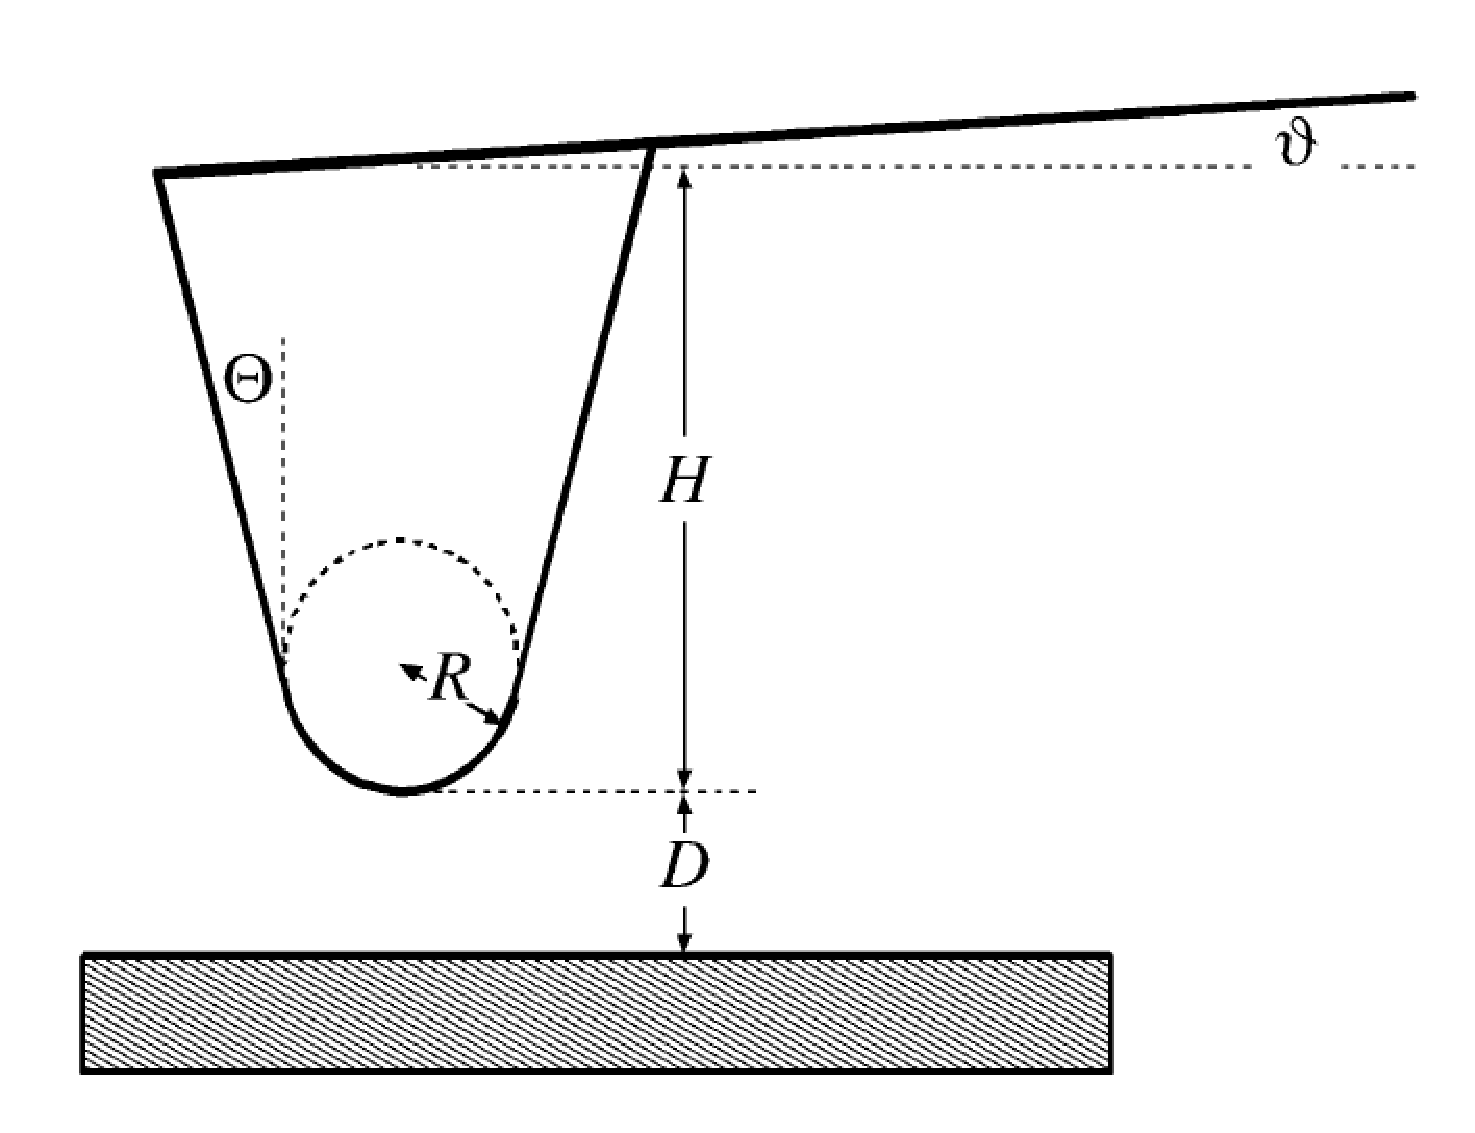
\includegraphics[width=0.45\columnwidth]{kepek/eps/tip-sample.eps}%
		\label{fig:tip-sample}}
		\caption{\scriptsize Az AFM apparátusa látható az (a) ábrán. A lázernyaláb
		a kantilever felületéről tükröződve egy fotódetektorra irányul. A tű pozícióját ez alapján nagy pontossággal ismerjük. A
		(b) ábrán a minta és a felette lévő tű modellje látható a kapacitás analitikus számításához.
		A tű $R$ sugarú $H$ magasságú és $D$ távolságra van a mintától. (Forrás: \cite{Butt20051})}
		\label{fig_sim}
	\end{figure}
	Az AFM felhasználása kontakt illetve kopogtató üzemmódú lehet. A kontakt mód során a
	felületen végighúzzuk a tűt és mérjük a $z$ irányű elmozdulását. Így képesek vagyunk a minta
	felületén lévő atomok elrendezéséről magasságtérkép adni.
	Kopogtató mód \cite{Martin1987} során a tűt elemeljük a mintától és $f$ frekvenciával rezegtetjük.
	A letapogatás során az  átlagos minta-tű távolságot a kontakt módú magasságtérkép felhasználásával
	konstans értéken tartjuk.
	A kantilever dinamikáját ismerve a rezegtetés frekvenciájának eltéréséből
	számítható a tűre ható erő. Ezen erő nagyságát két tényező befolyásolja:
	\begin{enumerate}[a)]
		\item a minta és a tű közötti feszültség,
		\item a minta felületi töltéssűrűség eloszlása.
	\end{enumerate}
	A cikkben a felületi töltéssűrűség mérését tekintjük célnak.
	A \cite{Butt1991Dec, Butt20051} szerint az erő a) komponensét a minta és a tű közötti
	kapacitásból a (\ref{eq:cap_force}) szerint származtathatjuk.
	\begin{equation}
	\label{eq:cap_force}
	F_{s} = -\frac{\ud E}{\ud D} = -\frac{\ud (CV^2 /2)}{\ud D} = -\frac12 \frac{\ud C}{\ud D} V^2
	\end{equation}
	Ha a minta pásztázása során ezen a) erőkomponens konstansnak mondható, tehát a felületi
	érdesség kicsi, akkor a töltéssűrűg mérésében állandó hibát okozva eliminálható.
	Az (\ref{eq:cap_force}) számításában a kritikus elem a kapacitás értéke, amit numerikus számítás
	mellőzése esetén a \cite{Hudlet1998} szerinti analitikus eredményt használhatjuk fel.
	A tű formályát a (\ref{fig:tip-sample} ábra) szerintinek veszi és a mintát sík felületünek
	feltételezi.
	Ezen utóbbi feltételezés legtöbb esetben helyénvaló, viszont a minta nagyfokú érdessége és a
	tű egyedi formálya esetén érvényét veszti. Ilyen esetben a kapacitás értéke mintáról
	mintára változik és állandó hiba helyett, a mérést zajként terheli.
	A kapacitás numerikus szimulációjával ezen zajt is ki lehet küszöbölni.
	Persze ezen szimulációt minden egyes mérési pontban el kell végezni, aminek a kivitelezése
	csak multiprocesszoros környezetben lehetséges elfogadható idő alatt.
	
\section{A feladat} \label{sec:feladat}
	A minta egy fémezett felület, aminek magasságtérképét mérések eredményeként ismerjük
	adott pontossággal.
	A mérések egy négyzetes háló felett történtek, amelynek a háló mindkét irányban
	$\delta_x = \delta_y \simeq 180 nm$ azonos felbontása, illetve a magasság $\delta_z \simeq 20nm$
	felbontása volt.
	A töltéssűrűség méréséhez szükséges második pásztázás során a tűt felemeljük és a mintához képest
	$V_{tu}$ potenciálra kapcsoljuk. Ezután a fémezett felülettől mindig azonos távolságra tartjuk és ezen 
	hosszú hegyes tűre ható erőt mérjük.
	\noindent
	\begin{center}
	Végső cél olyan szimulátor építése, amelynek segítségével közel valós időben 
	lehetséges felületmérés alapján a felületi töltéseloszlásról korrigált/pontosabb információt
	kapni.
	\end{center}
	
	A cikkben felhasznált mérési eredmény (\ref{fig:felulet}. ábra) egy
	$512\times512$ méretű szürkeárnyalatos *.tiff állomány, amely értéke $0-255$-ig terjed.
	
	\begin{figure}[!t]
		\centering
		\subfloat[Mérési eredmény]{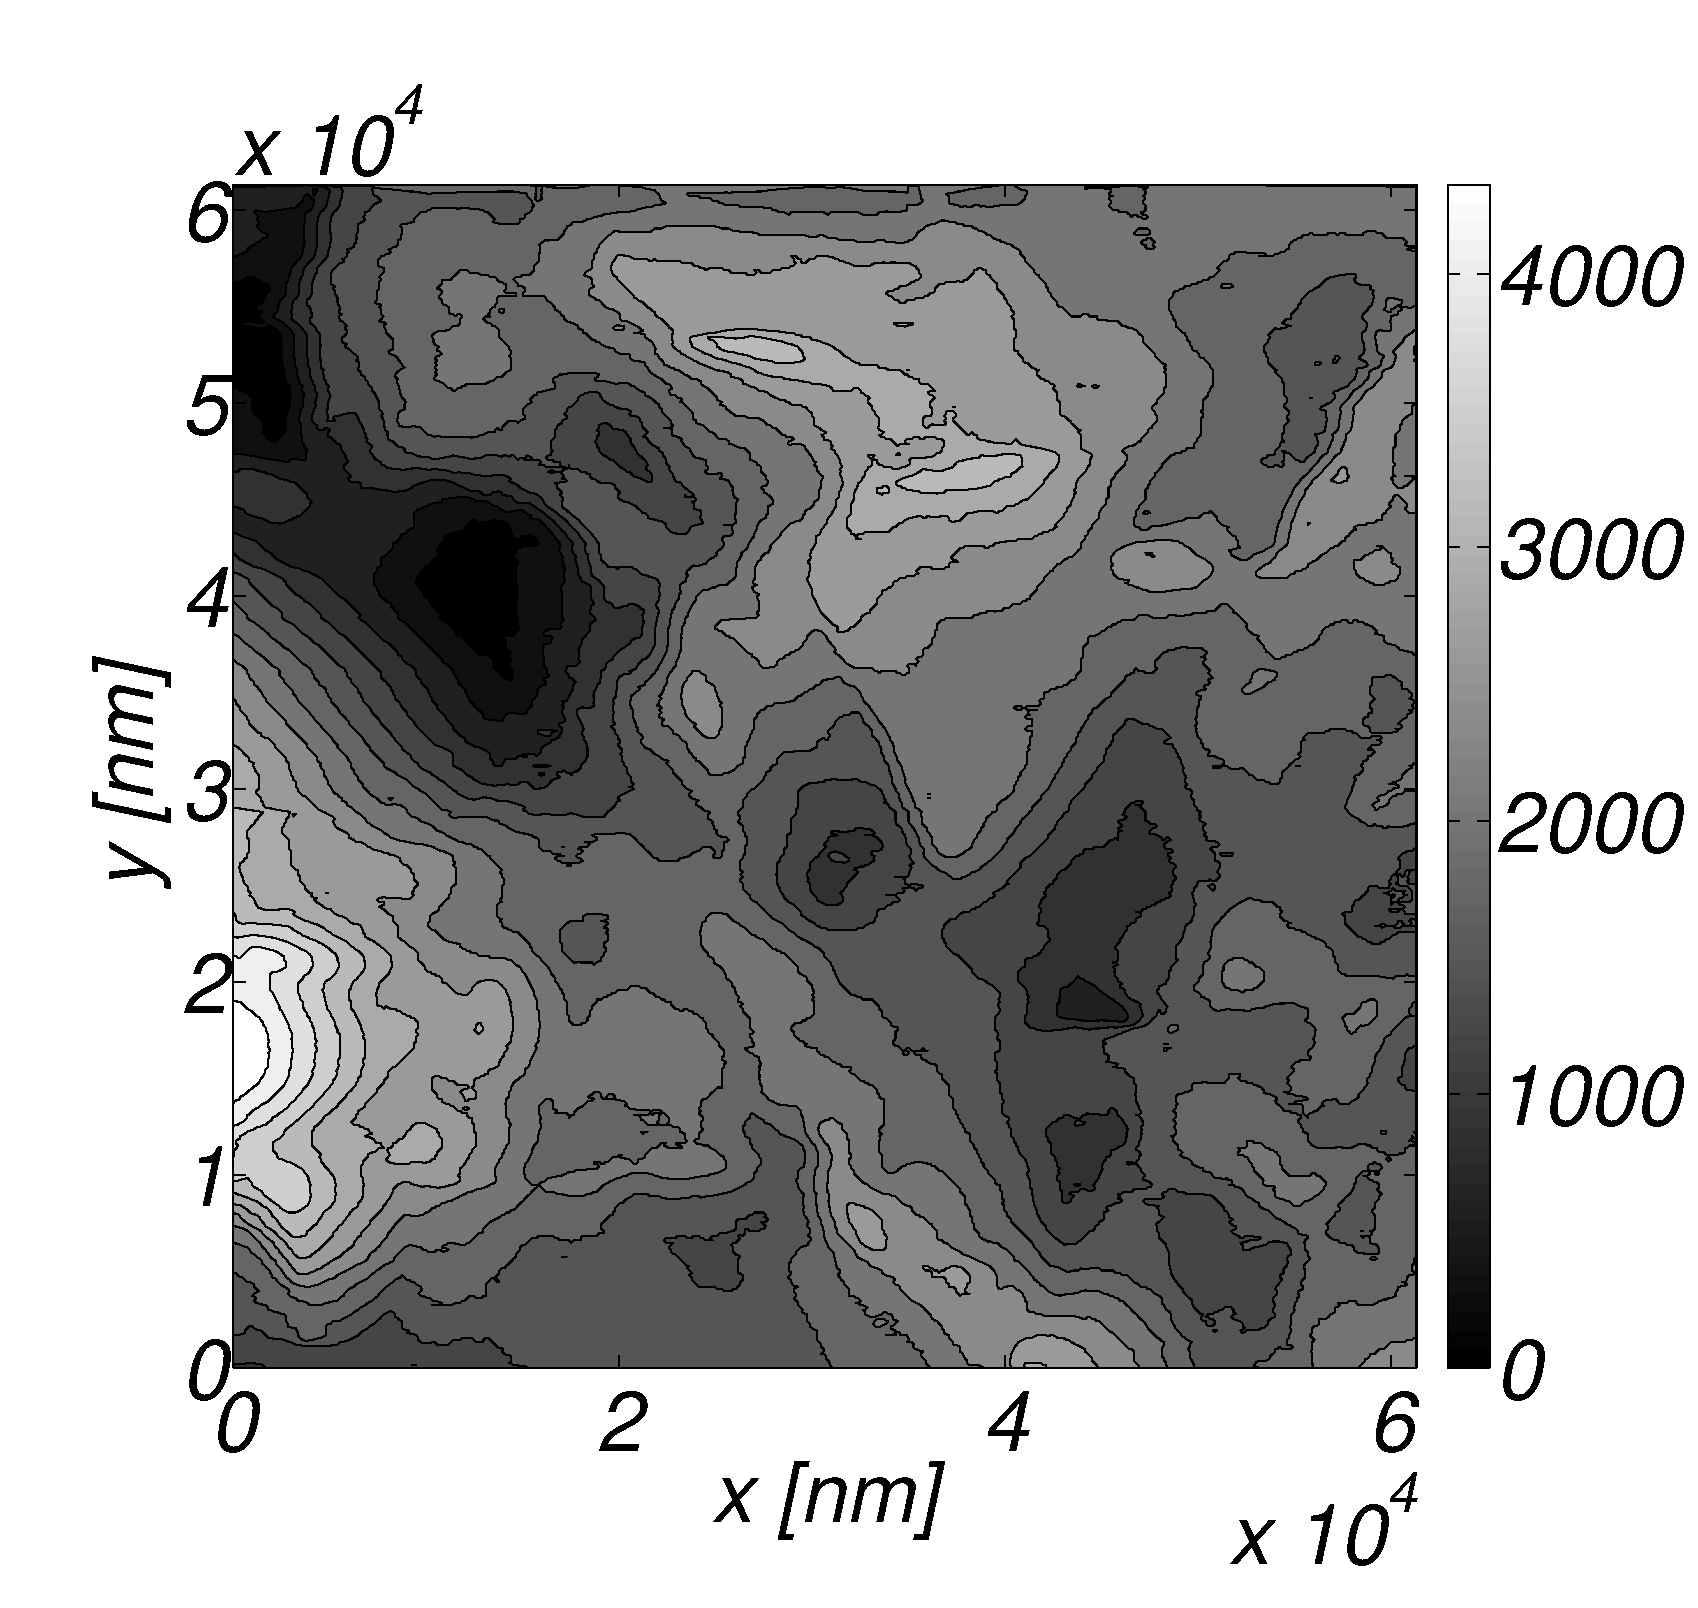
\includegraphics[width=0.5\columnwidth]{kepek/eps/newafm_total.eps}%
		\label{fig:afm_total}}
		\hfil
		\subfloat[Mérés részlete]{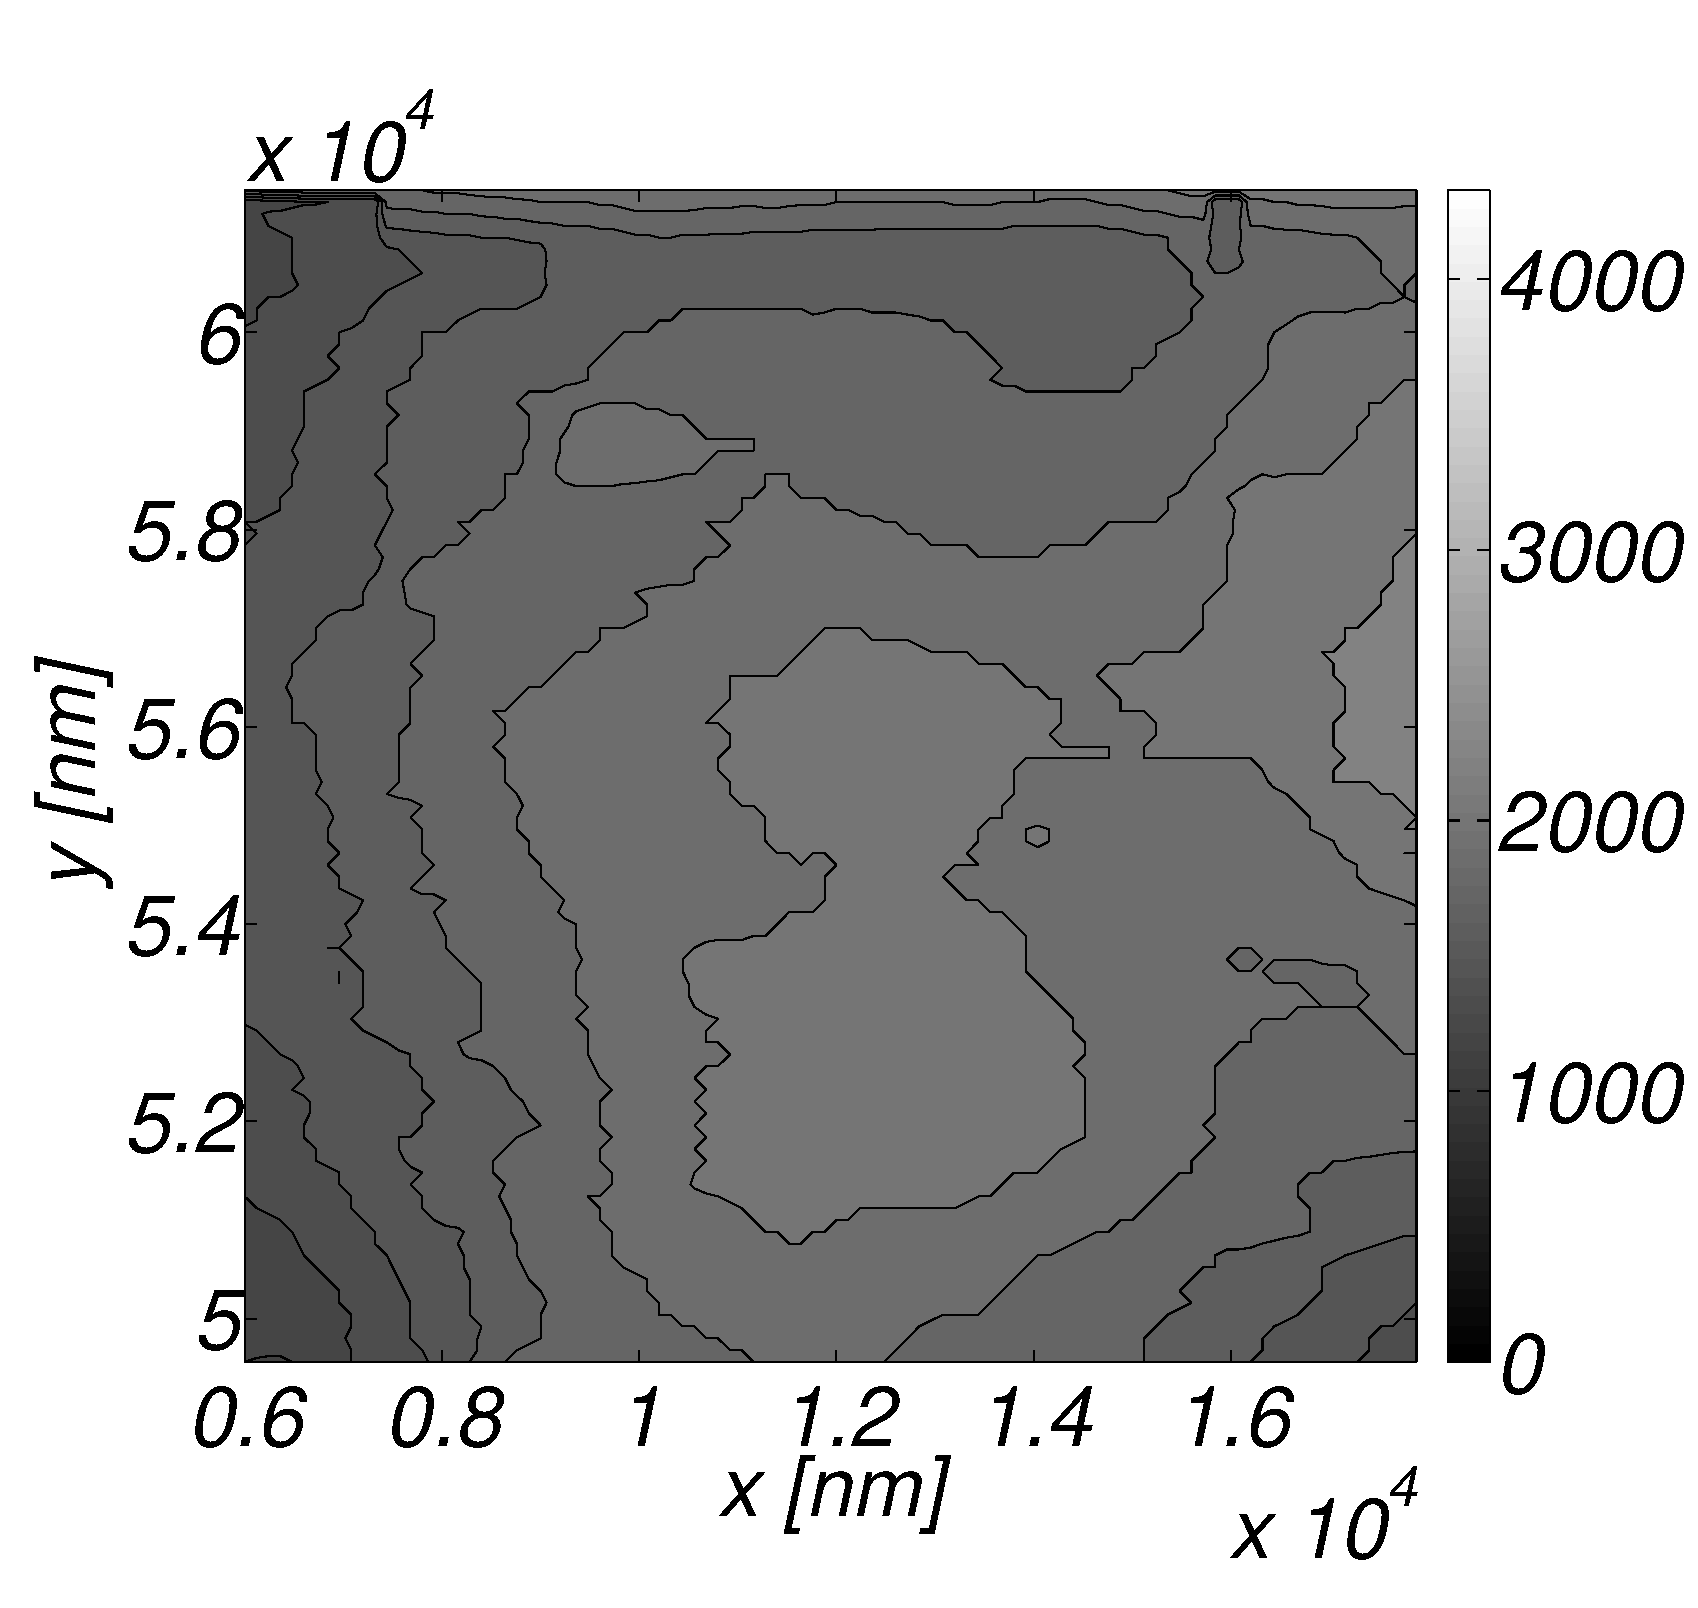
\includegraphics[width=0.5\columnwidth]{kepek/eps/newafm200.eps}%
		\label{fig:afm200}}
		\caption{\scriptsize Méréssel kapott magasságtérkép. Felbontás $d_x=d_y=120nm \ d_z=18.03nm$}
		\label{fig:felulet}
	\end{figure}
	
	
	
\section{Szimuláció}
\subsection{Fizikai probléma matematikai formalizálása}
	
	A megoldandó feladat egy elektrosztatikus feladat.
	A minta és a tű közötti térben nincsenek töltések, így itt a Poisson egyenlet helyett a
	Laplace-egyenlet \eqref{eq:laplace} érvényes.
	\begin{equation}\label{eq:laplace}
		\Delta V(x,y,z) = 0 
	\end{equation}
	Az egyenletet későbbiekben részletezett (\ref{sec:felepites}) megfontolások végett egy redukált
	3D-s téren oldjuk meg.
	Ezen 3D-s térre egy inhomogén ponthálót illesztünk, amelynek vízszintesen $d_x = d_y$,
	függőlegesen $d_z$ a felbontása. A függőleges felbontás megegyezik a használt AFM apparátus
	felbontásával $d_z = \delta_z$.
	Az így kapott térbeli háló minden pontjához hozzárendeljük az $V_{i,j,k} \simeq V(id_x,jd_y,kd_z)$
	potenciált.
	Dirichlet határfeltételek a felület fémezése, amely zérus potenciálú és az adott ($V_{tu}$)
	potenciálú  tű fémes felülete.
	A térnek a minta felületétől különböző határfelületén homogén Neumann feltételt alkalmazunk
	a szimmetriák (végtelen tér) és a töltésmentesség miatt.
	
	Az így adódó lineáris egyenletrendszer megoldására lehetséges direkt és iteratív megoldó
	algoritmusokat alkalmazni.
	%($1\leq i\leq i_{max}$, $1\leq j\leq j_{max}$, $1\leq k\leq k_{max}$). 
% 	Az alkalmazott interpoláció során a függőleges irányú felbontást is figyelembe véve 
	A párhuzamosítási szándékok miatt az iteratív megoldást választottuk, mivel a multiprocesszoros
	környezetek tipikusan kevés fajlagos-memóriával \footnote{Fajlagos alatt az egy szimulációra jutó
	memóriát értem. (Természetesen ezen szimulációk egyszerre futnak, így a fajlagos-memória
	akkumulálódik.)} rendelkeznek.
	Ekkor nem teljesen pontos megoldást kapunk, azonban gyorsabban juthatunk el a kívánt eredményhez.
	A számítási pontosság növelhető az iterációt leállító konvergencia követelmény keményebb
	megszabásával, ami persze több iterációt jelent.
	
	Az iteratív megoldás során a megoldás aktuális értékének kiszámításához az előző megoldásból indulunk ki.
	A \eqref{eq:laplace} egyenletben szereplő deriválást az elsőrendű Taylor közelítés alkalmazásával a
	\eqref{eq:it} 6-pontos sémát kapjuk.
	\begin{multline} \label{eq:it} 
		V_{ijk}^{n+1} = \\ \Delta_1 \cdot \left(V_{i-1,j,k}^n+V_{i+1,j,k}^n
		+V_{i,j-1,k}^n+V_{i,j+1,k}^n\right)+ \\
						\Delta_2 \cdot \left(V_{i,j,k-1}^n+V_{i,j,k+1}^n\right)
	\end{multline}
	ahol $V_{i,j,k}^n$ az az $n$-dik iterációs lépésben az $i,j,k$ indexü
	pontban mérhető potenciált jelöli, $\Delta_1$ a vízszintes felbontásból,
	$\Delta_2$ a függőleges felbontásból adódó állandó.
	%Az iterációs eljárás előnye, hogy implementációja egyszerűbb és a
	%\eqref{eq:2} szerinti ``simítás'' gyorsabb, mint a direkt megoldás.
	%Az iterációs eljárás előnye, hogy memóriaigénye kicsi a direkt megoldás során
	% adódó egyenletmegoldáshoz képest.
	%Hátránya hogy nem ad pontos választ egy lépésben.
	
% 	\begin{figure}[!ht]
% 		\centering
% 		\psfrag{ijk}{$(i,j,k)$}
% 		\psfrag{imjk}{$(i-1,j,k)$} 
% 		\psfrag{ipjk}{$(i+1,j,k)$}
% 		\psfrag{ijmk}{$(i,j-1,k)$} 
% 		\psfrag{ijpk}{$(i,j+1,k)$}
% 		\psfrag{d1}{$k_x$} 
% 		\psfrag{d2}{$k_y$} 
% 		\psfrag{d3}{$k_z$} 
% 		\psfrag{ijkm}{$(i,j,k-1)$} 
% 		\psfrag{ijkp}{$(i,j,k+1)$} 
% 		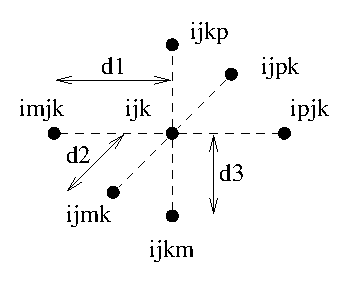
\includegraphics[width=0.95\columnwidth]{kepek/eps/sema.eps}
% 		\caption{\scriptsize Diszkretizálás során alkalmazott felosztás} 
% 	\end{figure}

	
% 	fi(idx,idy,idz) = KK1*(fip(idx-1,idy,idz)+fip(idx+1,idy,idz)+fip(idx,idy-1,idz)+fip(idx,idy+1,idz))+...
%               KK2*(fip(idx,idy,idz-1)+fip(idx,idy,idz+1))

\subsection{Szimuláció felépítése} \label{sec:felepites}
	
	A felületmérés során a vízszintes felbontás jóval kissebb, mint a függőleges felbontás, azaz a
	pontok vízszintes távolsága sokkal nagyobb a függőlegesnél $d_x=d_y \gg d_z$ (lásd \ref{sec:feladat}. rész).
	A Coulomb-kölcsönhatás a távolság négyzetével fordítottan arányos, így az előbb említettek értelmében egy mérési pont szomszédjait, pontosabban egy redukált
	környezetét szükséges csupán szimulálni (Másképpen megfogalmazva a vízszintes mérési pontok
	távolsága jóval nagyobb mint a Coulomb-kölcsönhatás effektív távolsága). Ezzel az elhanyagolással
	a feladat már numerikusan kezelhető méretűre csökken.
	
	Ezen módon egy mért pont $3\times3$-as környezetét vesszük figyelembe,
	a középső pont felett lévő elektródát (tűt) feltételezve.
	A szimulációs tér alsó felületét a mért magassági $3\times 3$ mintákból kell meghatároznunk.
	Mivel ezen pontokra úgy is tekinthetünk, mint a minta magasság-függvényének a mintavételezésével
	kapott mintáira, így a közbülső pontokat interpolációval (mozgó átlagolással) kapjuk meg.
	Az interpoláció $N_{ip}$ faktorával \footnote{$N_{ip}$-szeresére növeljük a pontok számát.}
	lehetséges a szimulációs tér vízszintes felbontását $d_x=d_y = \delta_x / N_{ip}$ megkapni.

	A szimulációk során a felület magasságának mérési adatait már ismertnek feltételezzük.
	A teljes magasságtérkép pontjait külön-külön vizsgáljuk.
	Egyetlen pontban a mérési eredmény kiszámításának lépései az alábbiak :
	
	\begin{enumerate}
		\item A pont körüli felület $3\times3$-as mérési részének megállapítása,
		\item Közbenső (virtuális) mérési pontokkal a belső felbontás növelése
		interpolációval,
		\item Szimulálandó tér méretének számítása,
		\item Direkt/iteratív megoldó algoritmussal a tér meghatározása, 
				a tűre ható erő számítása illetve a tű alatti töltésmennyiség számítása,
		\item Adatok mentése.
	\end{enumerate}
	

	
	
	 \section{A szimulátor bemutatása} 
	 A prototípus algoritmus fejlesztése MATLAB környezetben történt, ami később
	 referenciaként szolgál.
	 Alap MATLAB utasításokat használva több órát vesz igénybe a szimuláció
	 futtatása.
	 A MATLAB Parallel Toolbox-nak segítségével a szimulációt lehetséges
	 párhuzamosan több processzormagon futtatni. Ezzel párszoros sebesség
	 növekezés érhető el.
	 A következőkben magát az algoritmust és az OpenCL keretrendszerben történő
	 implementációját mutatjuk be.
	 Majd az eredmények bemutatása során kerül összevetésre a MATLAB
	 referencia, a MATLAB Parallel Toolbox segítséggel, az OpenCL processzoron és
	 az OpenCL GPU-n való futtatási ideje.
	
\subsection{A lépések részletezése} 
\subsubsection{Interpoláció}
	A korábban elmondottak alapján a felületet további virtuális pontokkal egészítjük ki.
	Az virtuális mérési pontokat a legegyszerűbb síklapos közelítéssel alkothatjuk meg,
	a magasságmérési felbontás figyelembevételével.
	A szimulátorban egy általánosabb módszert alkalmazunk,
	ami egy 2D-s mozgó átlagoló szűrővel való simítás.
	A szűrővel aluláteresztést tudunk elérni, ami a minta magasságának
	mintavételezése utáni rekonstrukcióját jelenti. Egy ilyen interpoláció
	eredményét láthatjuk a \ref{fig:33pont}. ábrán.
	
	\begin{figure}[!h]
		\centering
		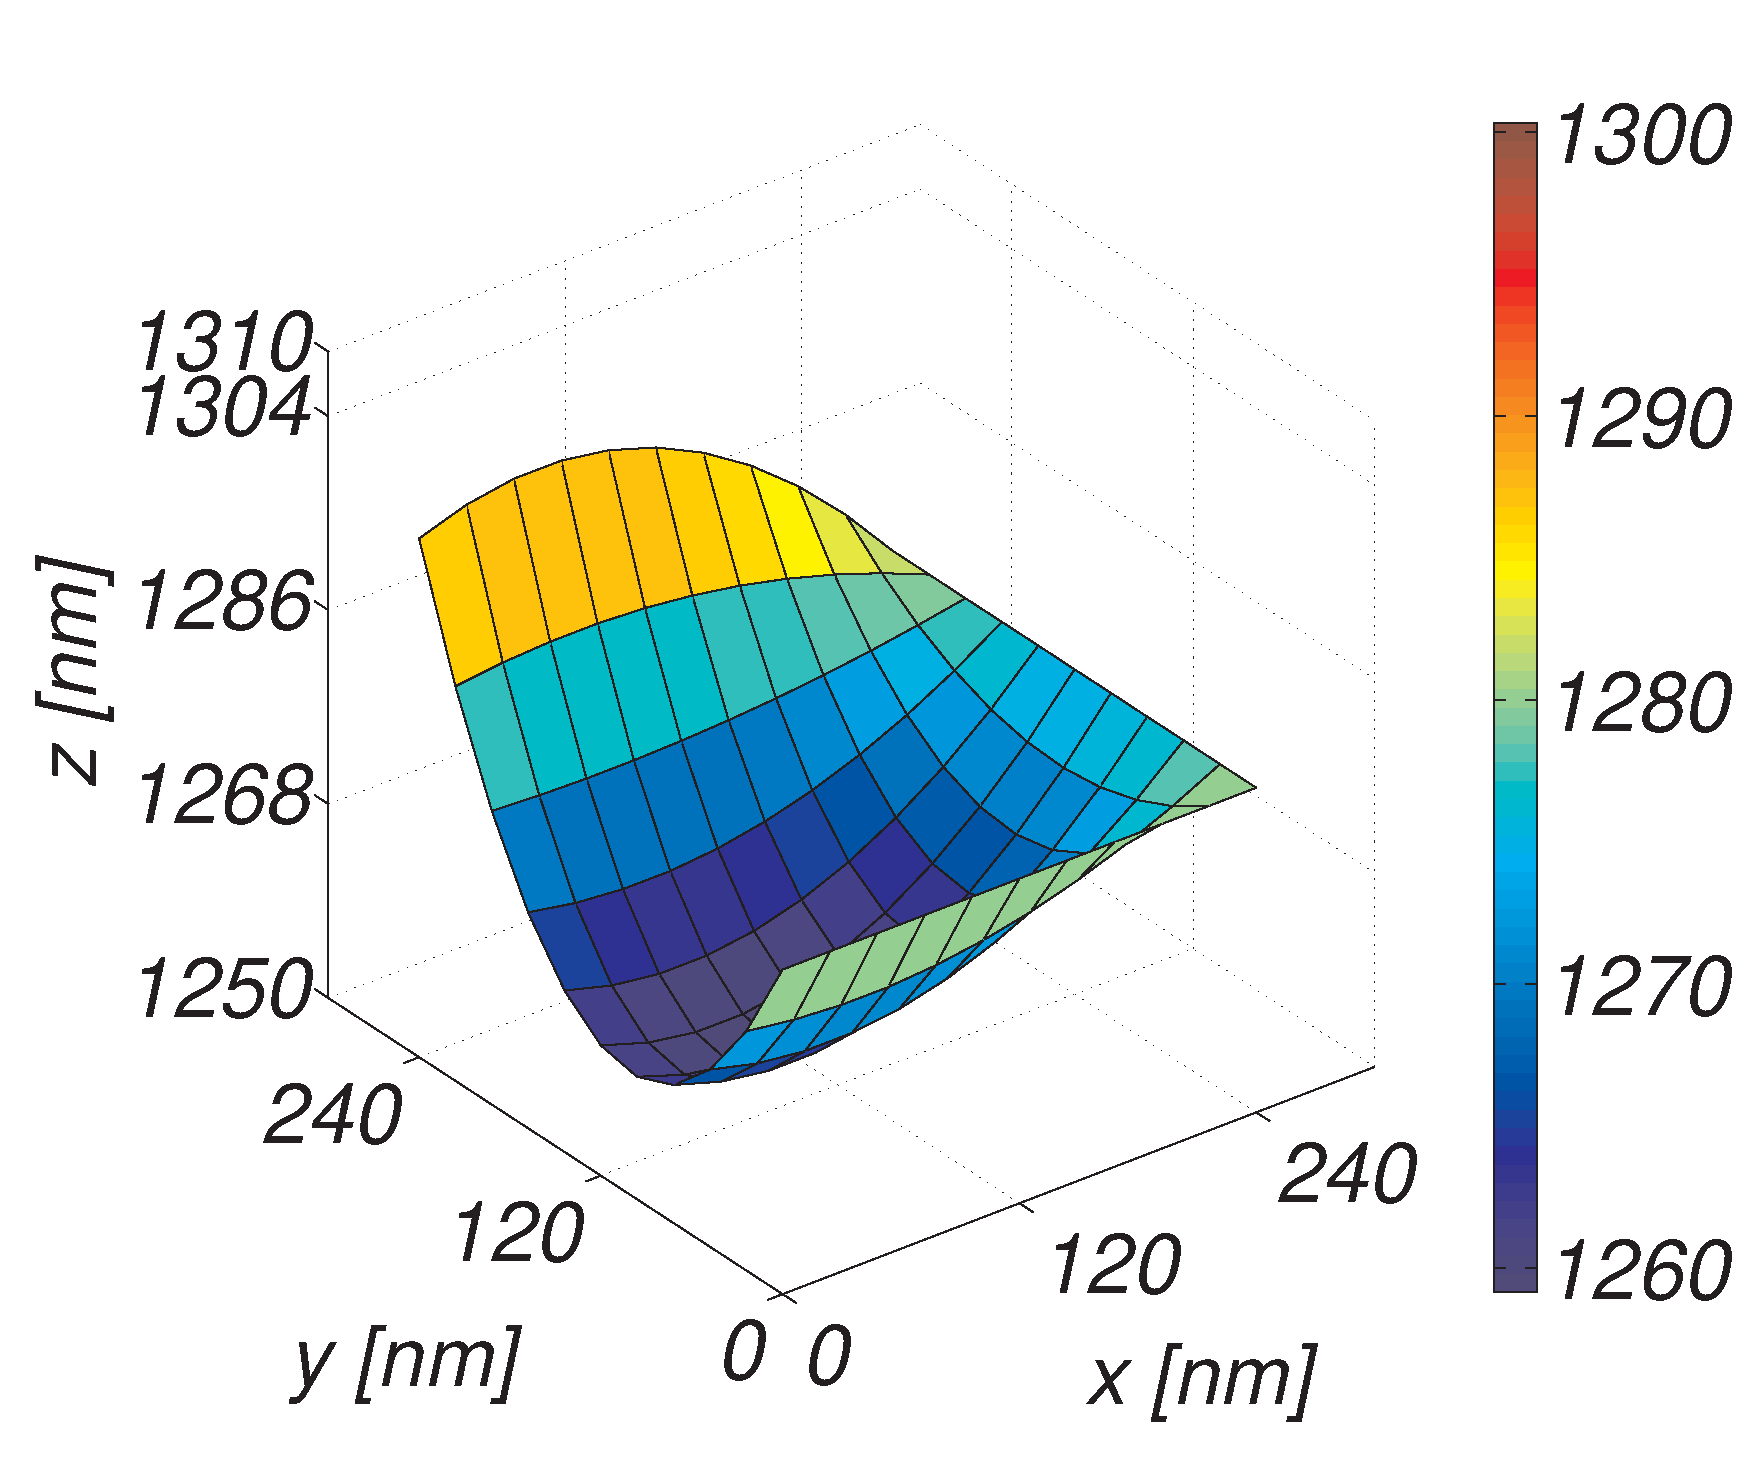
\includegraphics[width=0.8\columnwidth]{kepek/eps/3x3_interpol2.eps}
		\caption{\scriptsize $3\times3$ mérési pont $11\times11$ pontba való interpolációja}
		\label{fig:33pont}
	\end{figure}
	
\subsubsection{A szimulálandó tér mérete}
	\begin{figure}[!ht]
		\centering
		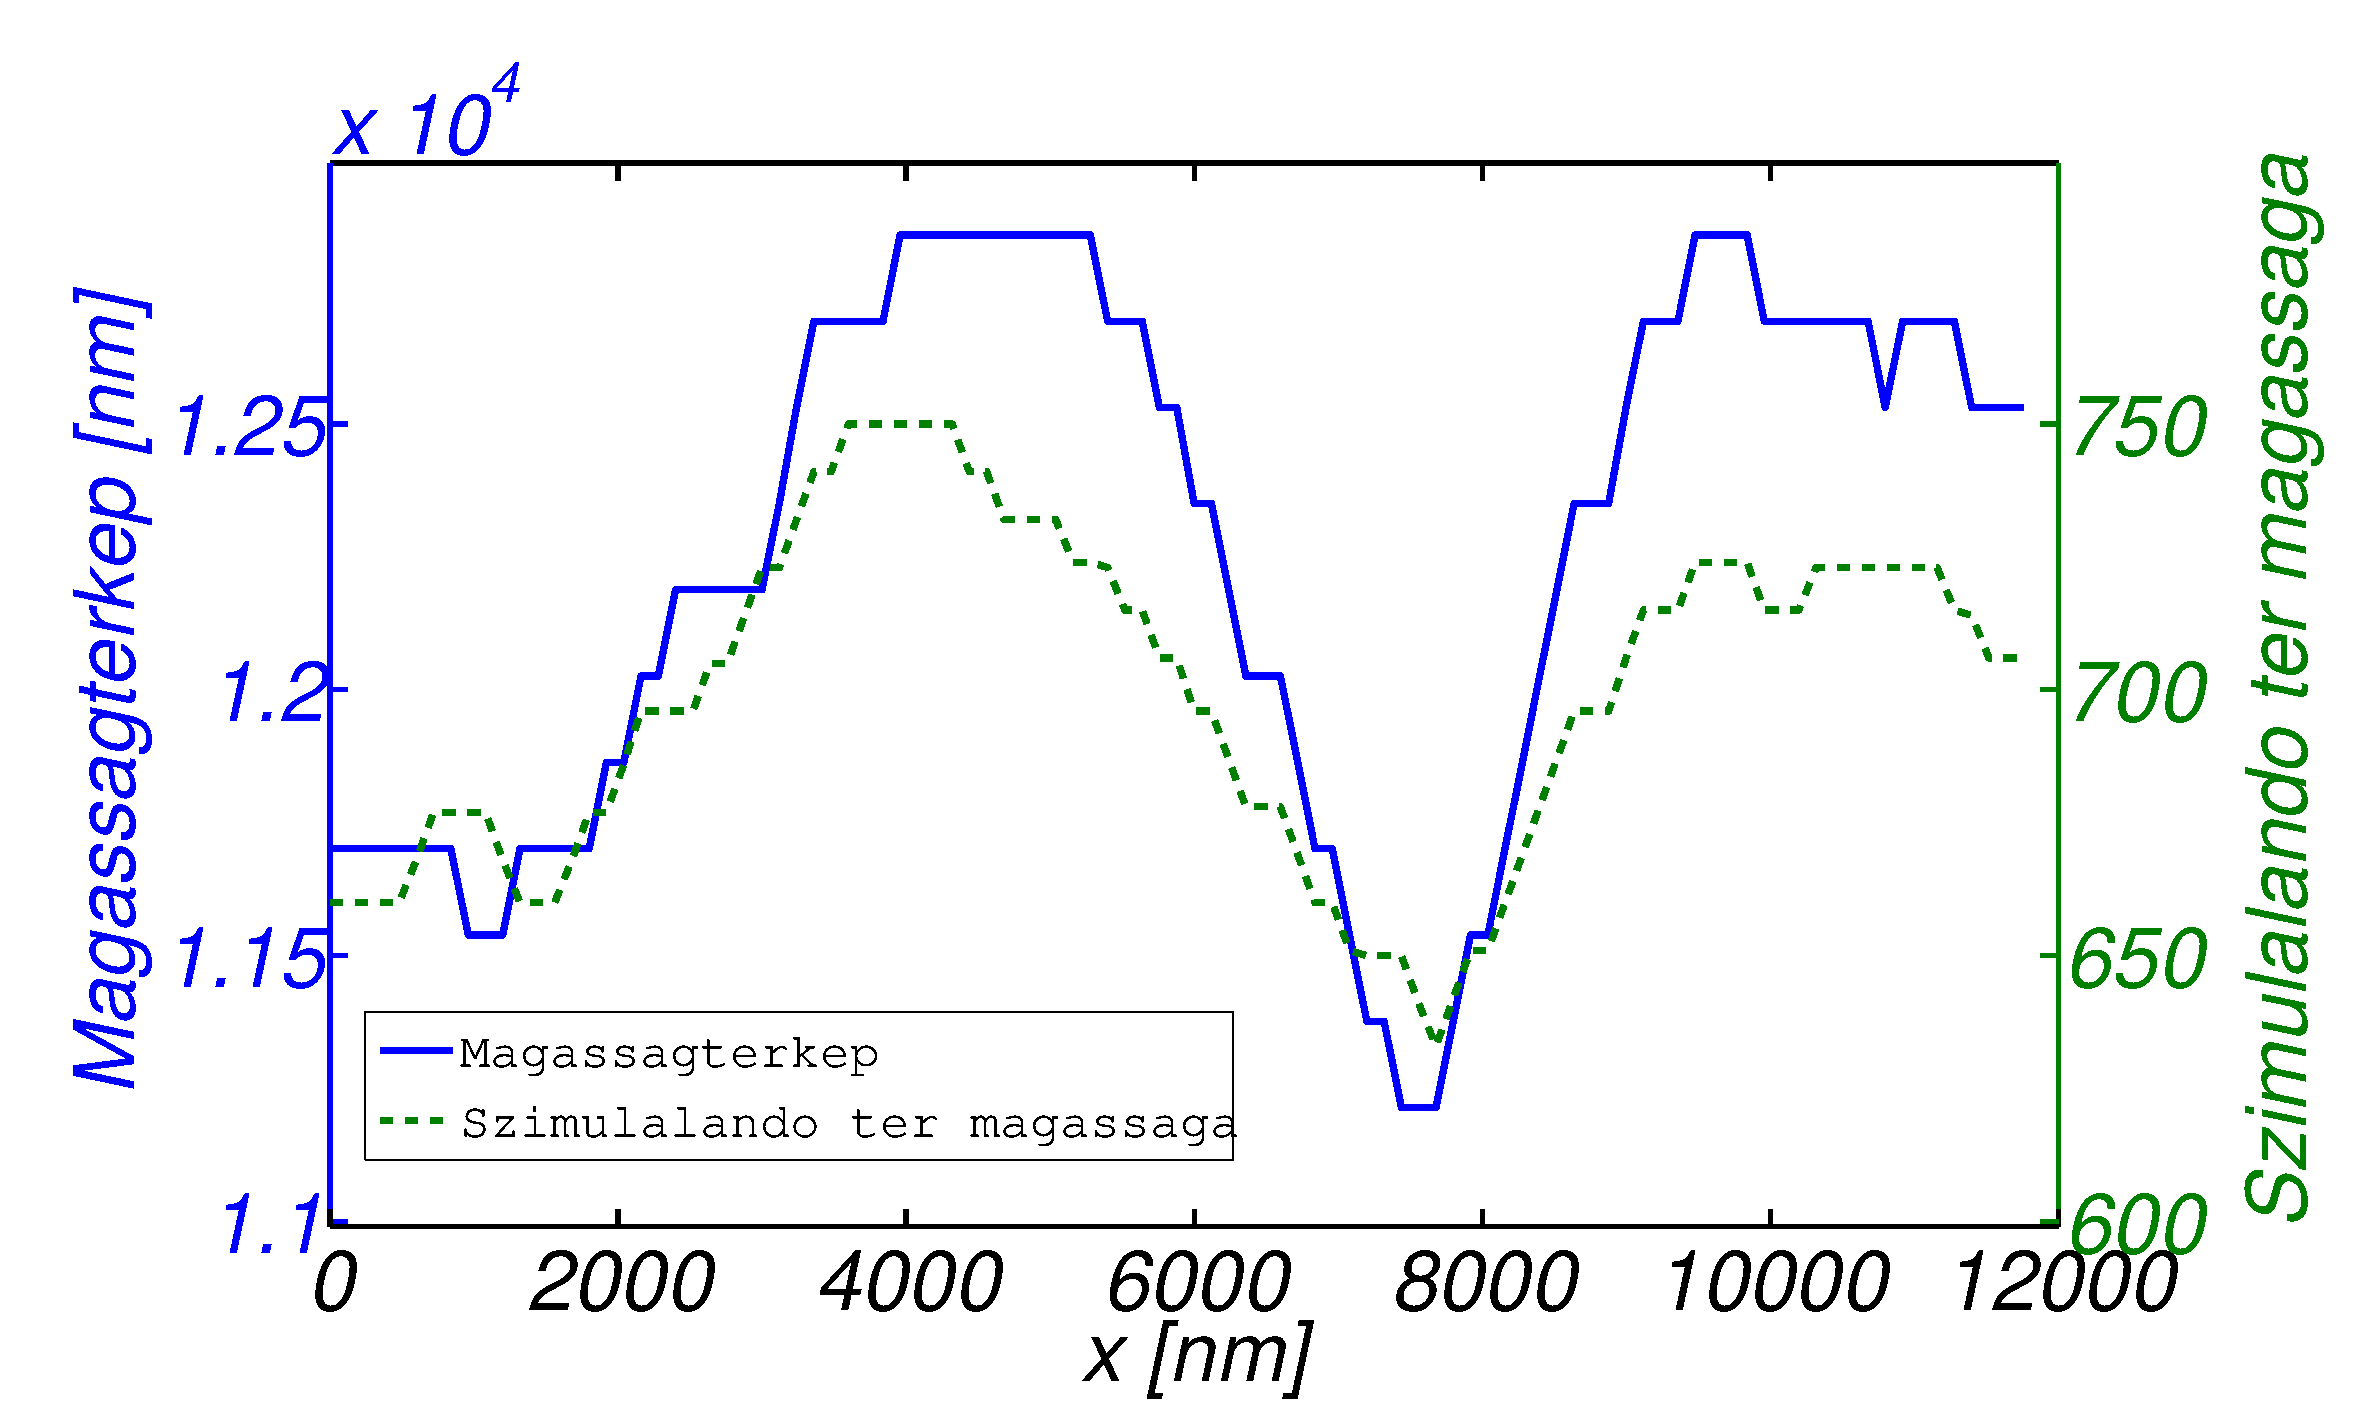
\includegraphics[width=0.7\columnwidth]{kepek/eps/numh_vonal.eps}%
		\caption{\scriptsize A mérési eredmény egy vonal menti részlete (folytonos vonal) és az ezen
		mérési pontokhoz számított szimulációs tér magassága (szaggatott-vonal)}
		\label{fig:numh} 
	\end{figure}
	
	A szimulálandó tér (hasáb) alapja adott az előzőleg említett interpolált felületként, míg a
	magassága nem. Ezt a következő két mennyiség közül a nagyobbikkal határoztuk meg:
	\begin{itemize}
		\item Középső pont fölött lévő tű közepének magassága,
		\item A ($3\times3$) környezet legalacsonyabb és legmagasabb pontjának
		különbsége.
	\end{itemize}
	A magasságtérkép egy vonalának részlete látható a \ref{fig:numh}. ábrán, 
	továbbá a szimulálandó tér (hasáb) magassága.
	
	\subsubsection{Iteratív megoldó algoritmus}
	Az iterációhoz a térháló pontjaihoz két mátrixot (tömbböt) rendelünk, ami a
	pontok potenciáljának aktuális ($\mathbf{U_{now}}$) és előző ($\mathbf{U_{prev}}$)
	értékeit tartalmazza.
	Az aktuális értékeket \eqref{eq:it} szerint számítjuk, majd az egész térre
	számítjuk az előzővel vett különbségének négyzetösszegét (normáját). E mérték
	képviseli a konvergencia szintjét, amit az iteráció során vizsgálva jutunk el a
	kívánt konvergencia szintre.
	Ha nem értük el a konvergencia szintet, akkor az előző két mátrixot
	felcserélve iterálunk tovább.
	
	\subsubsection{Adatok mentése}
	Tesztelhetőségi megfontolások végett a nem csak a tűre ható erőt (villamos
	térerősséget) exportáljuk, hanem a konvergencia szintjének változását és az
	interpolált felületet is. Az exportálandó menyiségek ``kis''
	mérete miatt egyszerű *.csv fájlként kerülnek mentésre. Ezen fájlok további
	poszt-processzálása MATLAB vagy munkalap kezelő szoftverrel is elvégezhető.
	
	\begin{table*}[!Ht]
		%\renewcommand{\arraystretch}{1.2}
		% if using array.sty, it might be a good idea to tweak the value of
		% \extrarowheight as needed to properly center the text within the cells
		\caption{\scriptsize OpenCL futási idő eredmények $12\times12$ mérési pontra}
		\label{table:openresult}
		% Some packages, such as MDW tools, offer better commands for making tables
		% than the plain LaTeX2e tabular which is used here.
		\centering
		\begin{tabular}{l|r|r|r}
		 & Globális memória & Lokális memória, ha befér & Lokális memória bufferelés\\ \hline
		\parbox{2.5cm}{Globális tranzakciók száma átlagosan} & $12 \times 12\times 32.3$
		& $12 \times 12 \times 32.3$ & $12 \times 12 \times 32.3$\\
		\parbox{2.5cm}{Lokális tranzakciók száma átlagosan} & 0 &
		$0.48 \times 12 \times 12 \times 30$ & $2.08 \times 12 \times12 \times 32.3$\\
		Futási idő & 5990 ms & 2530 ms & 510 ms\\
		Fajlagos futási idő & 410 ms & 170 ms & 3.5 ms 
		\end{tabular}
	\end{table*}

\subsection{OpenCL architektúrája}
	Az Open Computing Language (OpenCL) keretrendszer \cite{opencl} közös
	nyelvet, magas szintű programozási interfészt és hardware absztrakciót nyújt a fejlesztőknek
	adat- vagy feladat párhuzamos számítások gyorsítására különböző
	számítóegységen (CPU, GPU, FPGA, DSP, \ldots).
	Az OpenCL modellje a különböző ``device''-okra bontható, amik több ``compute unit''-ot
	(processzor-magot) tartalmaznak és ezeket heterogén módon kezeli. 
	
	\begin{figure}[!ht]
		\centering
		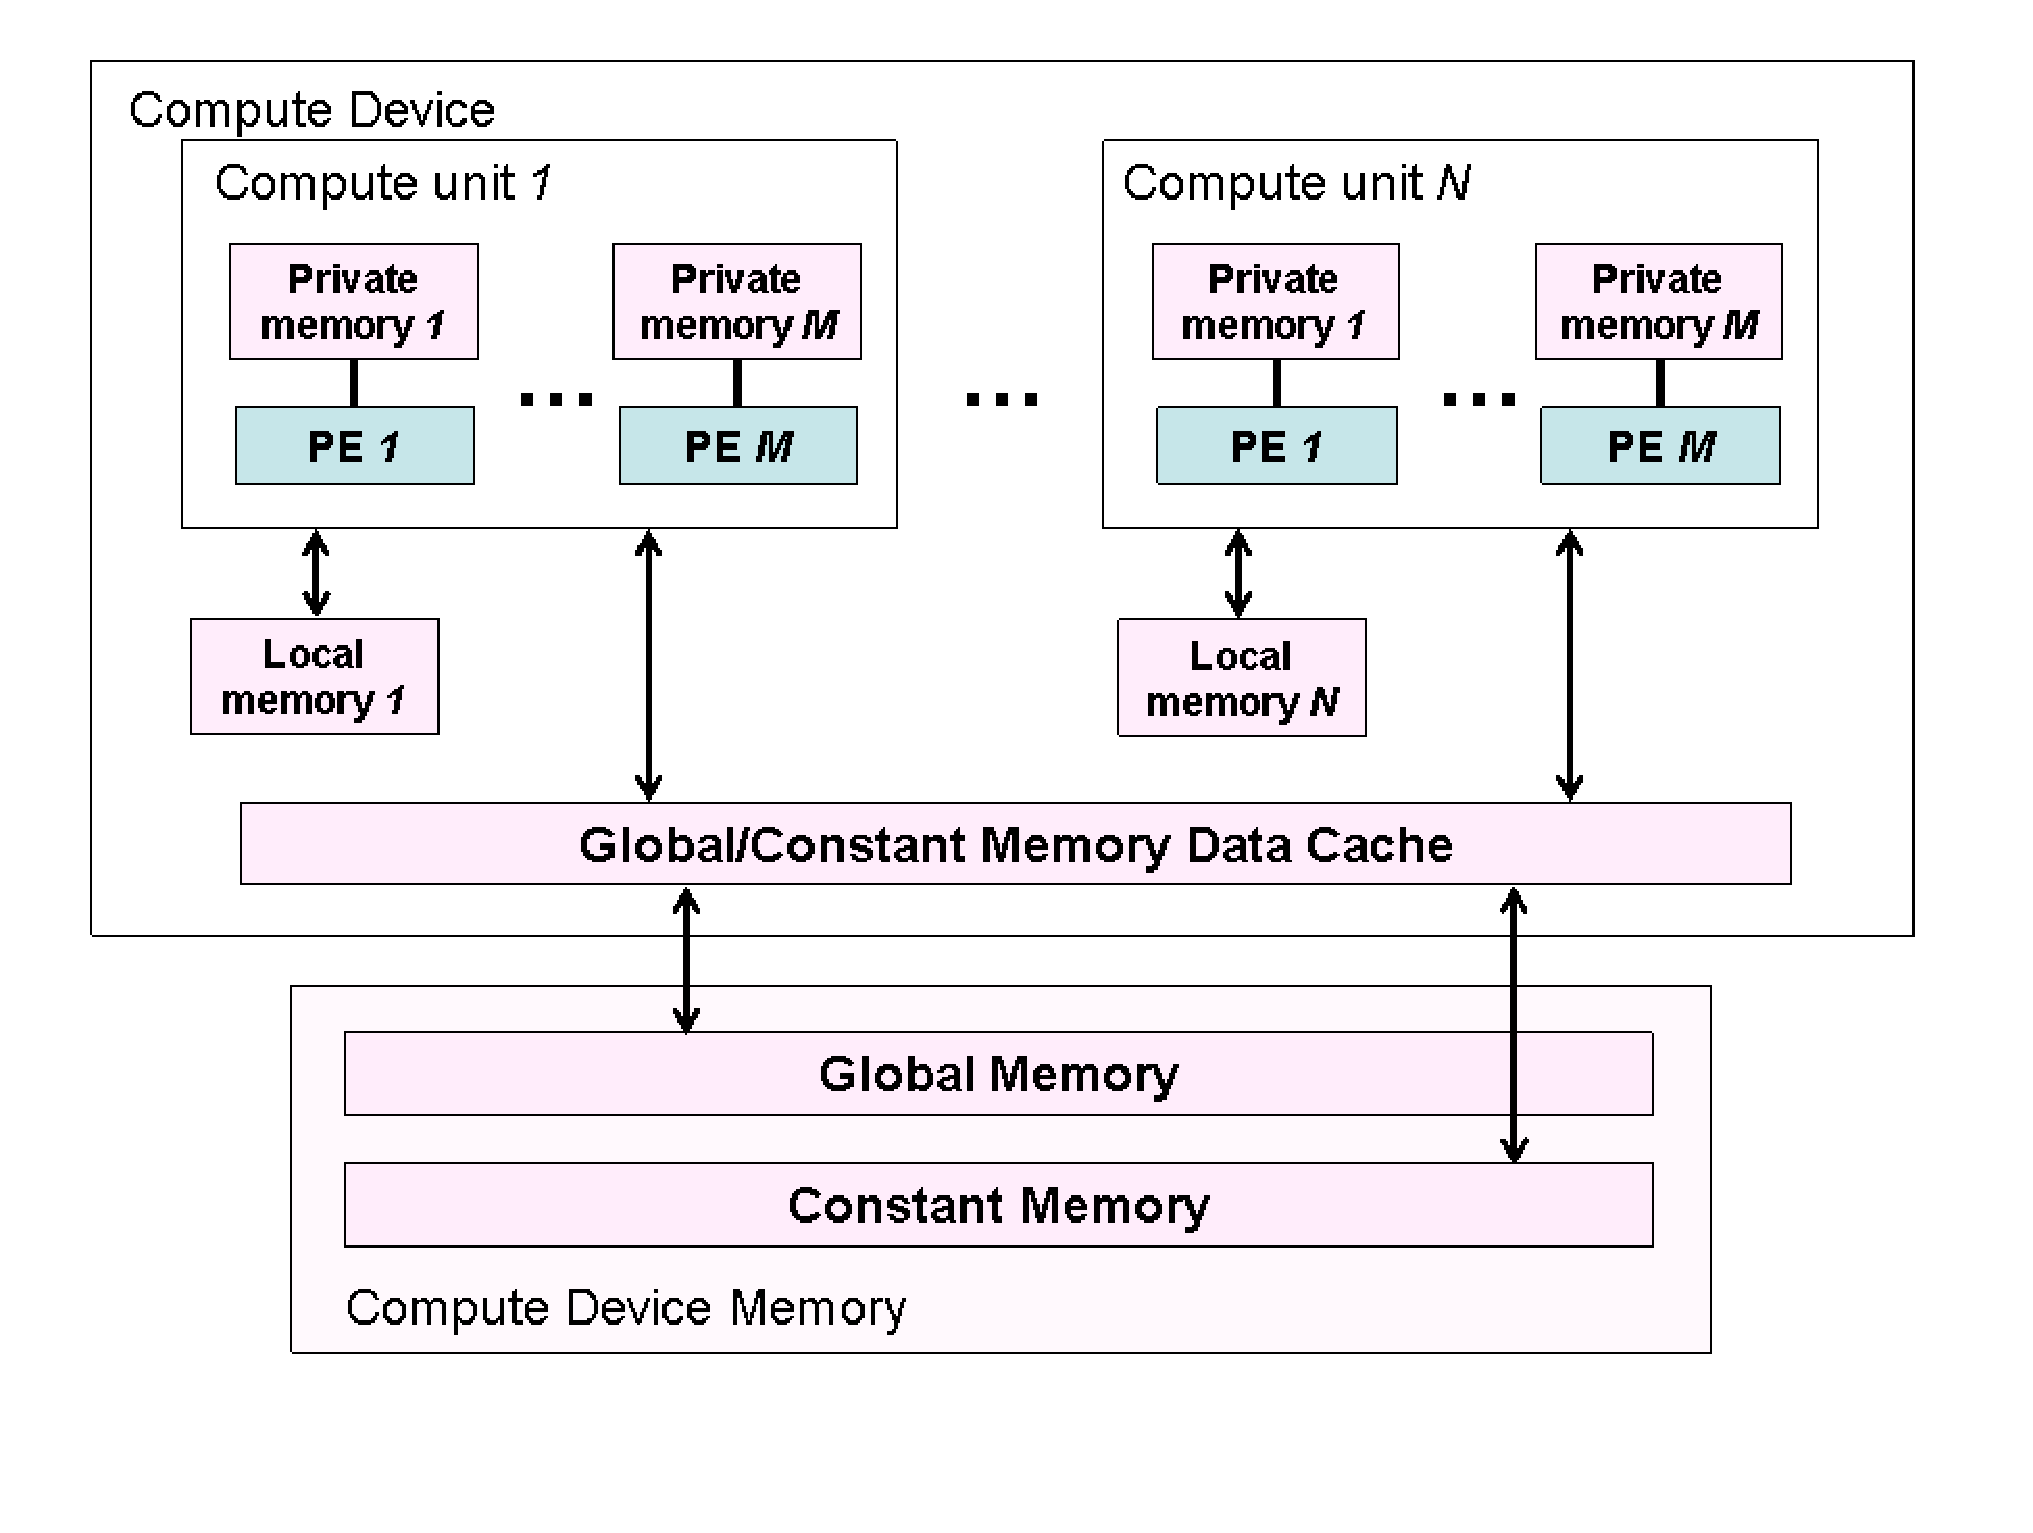
\includegraphics[width=0.7\columnwidth]{kepek/eps/opencl_device.eps}
		\caption{\scriptsize OpenCL ``device'' architektúra \cite{opencl}} 
		\label{fig:device} 
	\end{figure}
	
	A ``compute unit''-ok kiéheztetésének elkerülés végett (több ezer)
	``work-item'' virtuális osztozik rajta.
	Továbbá ezen ``work-item''-ek ``work-group''-okba vannak rendezve (később
	részletezett megfontolások végett).
	A ``compute unit'' kiéheztetését a ``device''-on található memória chipek lassúsága okozza.
	Ennek hárdveres megoldása a több szintű prediktív cache memória beiktatása a
	``compute unit'' és a külső memória közé.
	Mivel a bank szervezett külső memóriák hozzáférési ideje relatíve nagy
	így a memória szervezésére nagy hangsúlyt kell fektetni.
	
	Az OpenCL négy memória szintet különböztet meg, ami az
	\ref{table:mem} táblázatban és az \ref{fig:device}. ábrán látható.
	Ahhoz, hogy a rendszerben rejlő teljesítményt kiaknázzuk három fontos kérdést
	kell a szimulátor magjának implementálásakor megválaszolnunk:
	\begin{itemize}
		\item \textbf{Mennyit?}: Tisztában kell lennünk az aktuális
		memória fogyasztással és a szükséges memóriamérettel.
		\item \textbf{Honnan-hova?}: Fontos, hogy a lehető legközelebb legyen az adat
		a ``work-item''-hez.
		\item \textbf{Mikor?}: Mivel a memória művelet alatt a ``work-item'' nem
		dolgozik, így átadja a helyét egy másiknak. Ennek a megfelelő
		szinkronizációjával nagyobb kihasználtság érhető el (load balance).
	\end{itemize}
	
	\begin{table}[!h]
	\renewcommand{\arraystretch}{1.3}
	% if using array.sty, it might be a good idea to tweak the value of
	% \extrarowheight as needed to properly center the text within the cells
	\caption{\scriptsize OpenCL memória szintek}
	\label{table:mem}
	\centering
	% Some packages, such as MDW tools, offer better commands for making tables
	% than the plain LaTeX2e tabular which is used here.
	\resizebox{\columnwidth}{!}{
	\begin{tabular}{l|l|l|l|l}
			 & Global & Constant & Local & Private\\ \hline
		Host & Dinamikusan R/W & Din. R/W & Din. R/W & \\
		Kernel & R/W & Statikusan R & Satik. R/W & Statik. R/W\\
		Sebesség & Lassú & Gyors & Gyors & Regiszter\\
		Méret & $1$ Gbyte $<$ & $\sim64$ Kbyte& $\sim16$ Kbyte & $<1$ Kbyte
	\end{tabular}
	}
	\end{table}
	

	
	OpenCL keretrendszerben történő programozás során két programot kell írnunk.
	Az egyik a ``host''-on fut, ami elvégzi a probléma összeállítását, memória
	allokálását, argumentumok beállítását és a másik program a kernel meghívását a
	``device''-on.
	A kernel futása végeztével a ``host'' program kiolvassa a ``device''-ból
	a kívánt eredményt.
	
\subsection{Implementációhoz szükséges megfontolások}
	
	A következőkben egy kissebb teljesítményű notebook videókártyát veszek
	alapul a megfontolások demonstrálására. Ez az nVidia GeForce 330M, 
	575 MHz-en futó 48 CUDA core-al, 1024GB memóriával és
	OpenCL 1.0 kompatibilitással.
	A videókártya továbbiakban fontos paraméterei a \ref{table:vcard}. táblázatban
	látható.
	
	\begin{table}[!h]
	\renewcommand{\arraystretch}{1.3}
	% if using array.sty, it might be a good idea to tweak the value of
	% \extrarowheight as needed to properly center the text within the cells
	\caption{\scriptsize nVidia GeForce 330M OpenCL tulajdonságai}
	\label{table:vcard}
	\centering
	% Some packages, such as MDW tools, offer better commands for making tables
	% than the plain LaTeX2e tabular which is used here.
	\begin{tabular}{l|r}
		MAX\_COMPUTE\_UNITS & 6\\
		MAX\_WORK\_GROUP\_SIZES & 512 512 64\\
		GLOBAL\_MEM\_SIZE & 1073020928\\
		MAX\_CONSTANT\_BUFFER\_SIZE & 65536\\
		LOCAL\_MEM\_SIZE & 16384
	\end{tabular}
	\end{table}
	
	
	
	Ha a tér ahol a laplace egyenletet meg kell oldanunk nagyon nagy, akkor
	érdemes szétbontani kissebb alterekre és azokhoz rendelni egy-egy
	``work-item''-eket. Mivel a diszkrét Laplace egyenlet egy pontja a szomszédos
	pontokkal szoros kapcsolatban van, így az összefüggő ``work-item"-eket egy
	``work-group''-ba érdemes szervezni, mivel így az átlapolódó pontok értékét a
	szomszédos ``work-item'' is tudják írni és olvasni. Az ilyen típusú
	problémának méretét a MAX\_WORK\_GROUP\_SIZES tulajdonság korlátozza.
	
	Jelen esetben a mérési eredmény egy pontjához tartozó tér átlagosan
	$11\times11\times30$ pontból áll.
	Tehát a korábbi nem áll fenn és egyszerű megfeleltetéssel szétoszthatjuk a
	feladatot.
	A teljes tér $512\times512\times11\times11\times30$ méretű, ami $951k$ pont.
	A tárolásához single-precision mellett ennek a számnak a 4-szerese
	szükségeltetik byte-okban mérve. Mivel ez a videókártyán nem áll
	rendelkezésre, így szétbontjuk kissebb feladatrészekre.
	
	Ezen feladatrészek méretét egy paraméter állításával lehet változtati és az
	implementált algoritmus ettől generikusan függ.
	Emellett az interpoláció mértéke $N_{ip}$ is paraméterrel generikusan állítható.
	Az algoritmus generikusságát csupán a futási időben történő dinamikus memória
	allokációval lehetséges megvalósítani. A korábban említettek végett (\ref{table:mem} táblázat)
	az allokáció csak a ``host'' programban történhet.

\subsection{Memória szervezés}
	\subsubsection{Csak globális memória használata}
	Az algoritmus pszeudó kódjának direkt leképezése esetén a ``host''-on
	allokálunk memóriát a ``device'' globális memóriájában,
	majd a megfelelő adatokat ide másoljuk és a kernel is itt ír és olvas.
	A problémát a globális memória nagy hozzáférési ideje jelenti, ami miatt sok
	``work-item'' tétlenül a memóriára fog várakozni.
	Ilyenkor az egy mérési pontra vonatkoztatott szimulációs idő a
	referenciánál is lassabb.
	\subsubsection{Globális memória és adott esetben lokális memória használata}
	Kis erőfeszítéssel nagy javulást lehet elérni, ha a mérési ponthoz tartozó
	szimulációs tér éppen belefér a lokális memóriába.
	Tehát, mielőtt az \eqref{eq:it} szerinti iteratív megoldót futtatnánk elöször a
	globális memóriából a lokális memóriába töltjük át a kérdéses pontokat, majd
	számolunk rajta és a végén visszatöltjük a globális memóriába.
	E javítással a referenciával azonos sebességet tudunk elérni.
	\subsubsection{Globális memória és minden adódó alkalomkor a lokális memória használata}
	Nagyobb erőfeszítést igényel, hogy minden alkalammal a globális memóriával való kommunikációt a
	lokális memória közbeékelésével tegyük.
	Ezt úgy lehet felfogni, mintha a globális memóriát lokális memória méretű
	kvantumokban tudnám csak elérni.
	Ekkor nagy odafigyelést kíván a memóriacímzés megfelelő prgramozása, de
	eredményképp gyorsulás érhető el. \\
	
	\noindent
	\begin{center}
	Összegezve elmondható, hogy az aktuálisan használt adat tárolását a lehető
	legközelebb kell tartani a ``compute-unit''-hoz.
	\end{center}
	
	 \section{Eredmények} 
	\subsection{MATLAB implementációk}
	A referenciaként szolgáló MATLAB algoritmus lineáris programszervezést
	alkalmazva az elérhető fajlagos futási idő $\sim100 ms$.
	
	A kód minimális változtatásával elérhető a párhuzamos végrehajtás. Ezt a
	\texttt{for} ciklusok Parallel Toolbox beli \texttt{parfor} utasítására
	cserélve érhetjük el. 4 processzormaggal rendelkező PC esetén ilyenkor
	közel a negyedére csökken a futási idő.
	
	\subsection{OpenCL implementációk}
	OpenCL keretrendszer segítségével írt programot a GPU-n futtatva a
	\ref{table:openresult} táblázatban látható eredményeket kapjuk.
	Csupán a globális memóriát használva a referenciához képest romlik a
	teljesítmény. Ezt a videókártya prediktív cache nélküli kialakításának és a
	globális memórája okozta kiéheztetésnek tudhatjuk be.
	A lokális memória használata a futási időt drasztikusan le tudja
	csökkenteni, ami a korábban ismertetett memória szervezési gondolatok
	helyességét igazolja.
	 
	\begin{table*}[!t]
	\renewcommand{\arraystretch}{1.2}
	% if using array.sty, it might be a good idea to tweak the value of
	% \extrarowheight as needed to properly center the text within the cells
	\caption{\scriptsize OpenCL futási idő eredmények $12\times12$ mérési pontra}
	\label{table:openresult}
	% Some packages, such as MDW tools, offer better commands for making tables
	% than the plain LaTeX2e tabular which is used here.
	\centering
	\begin{tabular}{l|r|r|r}
	 & Globális memória & Lokális memória, ha befér & Lokális memória bufferelés\\ \hline
	\parbox{2.5cm}{Globális tranzakciók száma átlagosan} & $12 \times 12\times 32.3$
	& $12 \times 12 \times 32.3$ & $12 \times 12 \times 32.3$\\
	\parbox{2.5cm}{Lokális tranzakciók száma átlagosan} & 0 &
	$0.48 \times 12 \times 12 \times 30$ & $2.08 \times 12 \times12 \times 32.3$\\
	Futási idő & 5990 ms & 2530 ms & 510 ms\\
	Fajlagos futási idő & 410 ms & 170 ms & 3.5 ms 
	\end{tabular}
	\end{table*}
	
	\begin{figure*}[!t]
		\centering
		\subfloat[Mérési eredmény]{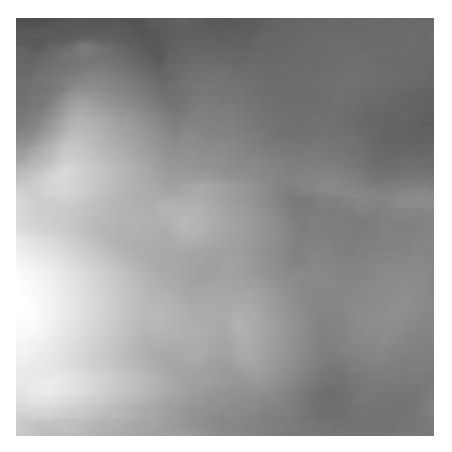
\includegraphics[width=0.45\columnwidth]{kepek/eps/afm200.eps}%
		\label{fig_first_case}}
		\hfil
		\subfloat[Szimulációs eredmény]{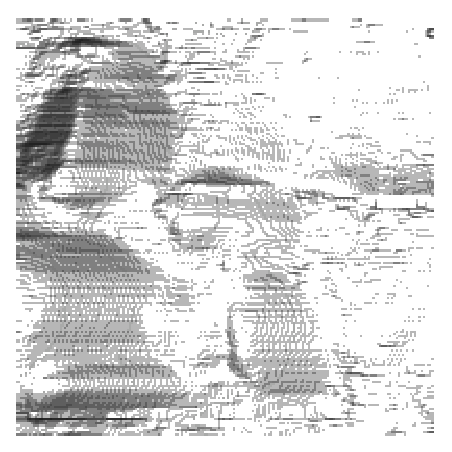
\includegraphics[width=0.45\columnwidth]{kepek/eps/efm200.eps}%
		\label{fig_second_case}}
		\caption{\scriptsize Méréssel kapott felület (balra) és szimulációval kapott töltéstérkép}
		\label{fig_sim}
	\end{figure*}
	

	
	\section{Összegzés}
	A cikkben összefoglaltam az AFM felületi töltéssűrűség méréstechnikáját, amiben azonosítottam a
	kapacitás értékének kritikus voltát. Ezidáig a kapacitás értékének a \cite{Hudlet1998,Butt20051}
	szerinti közelítéseket tartalmazó analitikus eredményt lehetett felhasználni.
	
	Feladatként ezen kapacitás értékét számító szimulátor építését tűztem ki, aminek elfogaható időn
	belül kell eredményt szolgáltatnia. A párhuzamosítás lehetősége triviálisan adódott.
	A hordozhatóság és a gyorsabb végrehajtás végett a szimulátort OpenCL 
	környezetben implementáltam, ami a szimulátor heterogén multiproszesszoros környezetben való
	futtatását lehetővé teszi.
	
	Az eredményeket ismertetve a szimulátor futási idejében látványos gyorsulást tapasztaltam, ami
	az érdesebb felületek esetén is elfogadhatóan pontos eredményt tud szolgáltatni. 
	
	A szimuláció felhasználásával történő töltéssűrűség származtatása még várat magára, ugyanígy ezen
	származtatás validálására való mérési összeállítás kidolgolgozása.
	A szimulátor magját képező lineáris egyenletrendszer iterációs megoldó
	konvergenciájának bizonyítása és az alternatív direkt megoldó vizsgálata is további feladat.

	
	
	
	\begin{thebibliography}{1}
	
	\bibitem{Web:khronos}
	The Khronos OpenCL Working Group, \emph{“OpenCL - The open stan-
	dard for parallel programming of heterogeneous systems.”} \\http://www.
	khronos.org/opencl/, 2014.
	
	
	
	\end{thebibliography}
	
\end{document}
